\chapter{Análise de Dados Categóricos}
\label{cap:categoricos}

Variáveis categóricas organizam observações em grupos, como meio de transporte, atividade realizada ou resposta sim/não. Neste capítulo, vamos construir uma tabela de contingência, comparar porcentagens e examinar a associação entre duas variáveis nominais. Depois, avançaremos para proporções, respostas pareadas e regressão logística binária. O ponto de partida é saber se cada linha do banco representa uma pessoa, um par de medidas ou uma contagem agregada.

\section{Tabela de contingência e denominadores}

O arquivo \href{https://github.com/erickfaria/apostilaJamovi/blob/main/dados/exemplo_frequencias.csv}{\texttt{dados/exemplo\_frequencias.csv}} contém quatro linhas que resumem \textbf{100 observações fictícias independentes}. A coluna \texttt{frequencia} informa quantas observações pertencem a cada combinação de \texttt{grupo} e \texttt{resultado}.

\begin{table}[H]
\centering
\caption{Contagens fictícias para praticar a análise de associação}
\begin{tabular}{lrrr}
\hline
Grupo & Sim & Não & Total \\
\hline
A & 30 & 20 & 50 \\
B & 15 & 35 & 50 \\
\hline
Total & 45 & 55 & 100 \\
\hline
\end{tabular}
\label{tab:contingencia-exemplo}
\end{table}

Entre as 50 observações do grupo A, $30/50=60\%$ têm resultado Sim. No grupo B, são $15/50=30\%$. Essas são \textbf{porcentagens por linha}. Já $30/45\approx66{,}7\%$ responde a outra pergunta: entre todos os resultados Sim, qual fração pertence ao grupo A? Essa é uma porcentagem por coluna. Indique o denominador em tabelas, figuras e texto.

\begin{figure}[H]
\centering
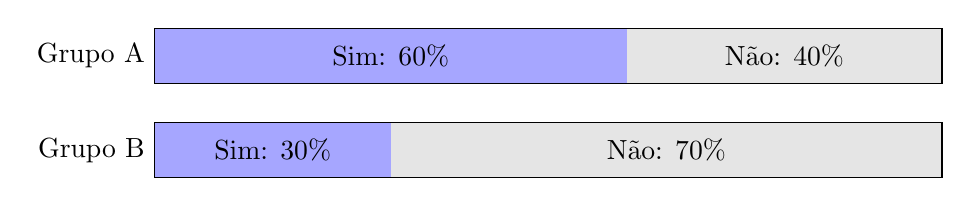
\begin{tikzpicture}[x=1cm,y=1cm]
  \node[left] at (0,1.5) {Grupo A};
  \node[left] at (0,0.3) {Grupo B};
  \fill[blue!35] (0,1.15) rectangle (6,1.85);
  \fill[gray!20] (6,1.15) rectangle (10,1.85);
  \draw (0,1.15) rectangle (10,1.85);
  \fill[blue!35] (0,-0.05) rectangle (3,0.65);
  \fill[gray!20] (3,-0.05) rectangle (10,0.65);
  \draw (0,-0.05) rectangle (10,0.65);
  \node at (3,1.5) {Sim: 60\%};
  \node at (8,1.5) {Não: 40\%};
  \node at (1.5,0.3) {Sim: 30\%};
  \node at (6.5,0.3) {Não: 70\%};
\end{tikzpicture}
\caption{Composição percentual dentro de cada grupo; cada barra representa 100\% de sua linha. Elaboração própria.}
\label{fig:proporcoes-grupos}
\end{figure}

\section{Configurando a tabela no jamovi}

\begin{enumerate}
  \item Abra o CSV e configure \texttt{grupo} e \texttt{resultado} como nominais. A coluna \texttt{frequencia} contém contagens inteiras.
  \item Acesse \textbf{Análises $\rightarrow$ Frequências (Frequencies) $\rightarrow$ Tabelas de contingência (Contingency Tables) $\rightarrow$ Amostras independentes (Independent Samples)}.
  \item Atribua \texttt{grupo} a \textbf{Linhas (Rows)}, \texttt{resultado} a \textbf{Colunas (Columns)} e \texttt{frequencia} a \textbf{Contagens (Counts)}.
  \item Solicite as contagens observadas, as esperadas e as porcentagens por linha. Confira que o total é $100$.
\end{enumerate}

A documentação oficial descreve o uso de uma coluna de contagens e as opções para porcentagens, qui-quadrado, Fisher e medidas de associação \parencite{JamoviContingencia}. Se cada linha do seu banco representar uma única pessoa, deixe \textbf{Contagens} vazio: não use o identificador da pessoa como peso.

\begin{tcolorbox}[colback=white,colframe=green,title={Dica de Conteúdo}]
As quatro linhas do arquivo não são quatro participantes. Sem atribuir \texttt{frequencia} ao campo de contagens, você analisará combinações de categorias em vez das 100 observações resumidas. Sempre confira os totais antes de interpretar o teste.
\end{tcolorbox}

\section{Teste qui-quadrado de independência}

A hipótese nula afirma que as duas variáveis são independentes na população modelada. Para cada célula, calculamos uma frequência esperada sob essa hipótese:
\[
E_{ij}=\frac{(\text{total da linha }i)(\text{total da coluna }j)}{n}.
\]
Na célula A/Sim, o valor esperado é $50\times45/100=22{,}5$. Na célula A/Não, é $27{,}5$. Os mesmos valores esperados se repetem na linha B, porque os dois totais de linha são iguais.

A estatística de Pearson compara contagens observadas $O_{ij}$ e esperadas $E_{ij}$:
\[
\chi^2=\sum_i\sum_j\frac{(O_{ij}-E_{ij})^2}{E_{ij}},
\qquad gl=(r-1)(c-1),
\]
em que $r$ e $c$ são o número de linhas e colunas. Para nossa tabela $2\times2$, selecione o qui-quadrado de Pearson \textbf{sem correção de continuidade}. Você deve encontrar aproximadamente $\chi^2(1)=9{,}091$ e $p=0{,}00257$. Se selecionar a correção de continuidade, o resultado numérico será outro; identifique a opção usada.

No exemplo, os percentuais observados diferem e o teste é incompatível com a independência ao nível de 5\%, sob as condições consideradas. O teste não estabelece que pertencer ao grupo A cause o resultado Sim.

\subsection{Quando examinar Fisher e a estrutura do estudo}

A aproximação qui-quadrado exige atenção às frequências \textbf{esperadas}, não apenas ao tamanho total ou à presença de uma contagem observada pequena. Em tabelas $2\times2$ com frequências esperadas muito baixas, considere o teste exato de Fisher e justifique o procedimento. Para a tabela da apostila, Fisher bilateral produz aproximadamente $p=0{,}00464$; esse valor não precisa coincidir com o de Pearson.

Cada observação precisa contribuir de modo compatível com a hipótese de independência. Se a mesma pessoa responde antes e depois a uma pergunta binária, os registros são pareados. O teste de McNemar trata uma pergunta desse tipo; a tabela de grupos independentes discutida aqui não é uma substituição adequada.

\subsection{Resíduos: onde estão os afastamentos?}

Uma estatística global soma contribuições de todas as células. O resíduo de Pearson de uma célula é:
\[
r_{ij}=\frac{O_{ij}-E_{ij}}{\sqrt{E_{ij}}}.
\]
Em A/Sim, ele vale $(30-22{,}5)/\sqrt{22{,}5}\approx1{,}581$. O sinal positivo indica mais respostas Sim do que o esperado sob independência; o negativo, menos. Os quadrados desses resíduos somam o qui-quadrado de Pearson sem correção.

Também podemos considerar um resíduo padronizado \textbf{ajustado}, levando em conta a estimação das margens. Para uma tabela de independência, uma expressão é:
\[
z_{ij}=\frac{O_{ij}-E_{ij}}
{\sqrt{E_{ij}(1-p_{i+})(1-p_{+j})}},
\]
em que $p_{i+}$ e $p_{+j}$ são as proporções marginais da linha e da coluna. A documentação de \texttt{chisq.test} do R distingue resíduos de Pearson e resíduos padronizados \parencite{RQuiQuadrado}. Esses nomes podem variar entre programas: confira a fórmula antes de comparar números.

\begin{figure}[H]
\centering
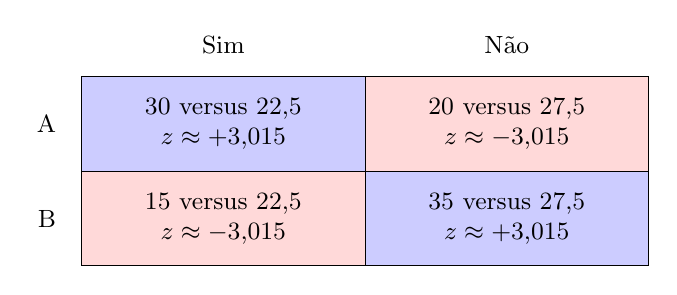
\begin{tikzpicture}[x=1cm,y=1cm,every node/.style={font=\small,align=center}]
  \node at (1.8,2.8) {Sim};
  \node at (5.4,2.8) {Não};
  \node[left] at (-0.2,1.8) {A};
  \node[left] at (-0.2,0.6) {B};
  \fill[blue!20] (0,1.2) rectangle (3.6,2.4);
  \fill[red!15] (3.6,1.2) rectangle (7.2,2.4);
  \fill[red!15] (0,0) rectangle (3.6,1.2);
  \fill[blue!20] (3.6,0) rectangle (7.2,1.2);
  \draw (0,0) rectangle (7.2,2.4);
  \draw (3.6,0) -- (3.6,2.4);
  \draw (0,1.2) -- (7.2,1.2);
  \node at (1.8,1.8) {$30$ versus $22{,}5$\\$z\approx+3{,}015$};
  \node at (5.4,1.8) {$20$ versus $27{,}5$\\$z\approx-3{,}015$};
  \node at (1.8,0.6) {$15$ versus $22{,}5$\\$z\approx-3{,}015$};
  \node at (5.4,0.6) {$35$ versus $27{,}5$\\$z\approx+3{,}015$};
\end{tikzpicture}
\caption{Contagens observadas versus esperadas e resíduos ajustados da tabela A/B. Azul indica excesso e vermelho, falta em relação ao modelo de independência. As quatro células não representam quatro descobertas independentes. Elaboração própria.}
\label{fig:residuos-contingencia}
\end{figure}

Nesta tabela $2\times2$, margens fixadas deixam apenas um grau de liberdade: o excesso em uma célula determina os sinais das demais. Em tabelas maiores, uma inspeção dos resíduos ajuda a descrever o padrão, mas decisões por célula também precisam considerar a multiplicidade. Um corte como $|z|>1{,}96$ não fornece, sozinho, controle simultâneo de todas as comparações.

Essas contas usam \textbf{frequências de observações independentes}. Pesos de uma amostra complexa não são automaticamente contagens de repetições independentes; a soma dos pesos pode ser um total populacional estimado. Se os pesos vierem de um plano amostral com estratos e conglomerados, use procedimentos compatíveis com esse plano, em vez de inserir os pesos no campo Contagens e interpretar o total como tamanho amostral.

\section{Magnitude da associação}

O valor de $p$ não quantifica o tamanho da associação. Uma opção para tabelas nominais é o V de Cramér:
\[
V=\sqrt{\frac{\chi^2}{n\,\min(r-1,c-1)}}.
\]
No exemplo, $V=\sqrt{9{,}091/100}\approx0{,}302$. A medida não indica a direção da associação; para compreendê-la, examine os percentuais da tabela. Sua importância depende também da pergunta e do contexto.

\subsection{Razão de chances não é razão de probabilidades}

Para um resultado com probabilidade $p$, a chance, ou \textit{odds}, é $p/(1-p)$. No grupo A, a chance observada de Sim é $30/20=1{,}5$; no grupo B, é $15/35\approx0{,}429$. A razão de chances de A em relação a B é:
\[
OR=\frac{30/20}{15/35}=3{,}5.
\]
Isso não significa que a probabilidade de Sim seja 3,5 vezes maior. A razão entre as proporções observadas é $0{,}60/0{,}30=2$. A interpretação como risco, prevalência ou outra medida depende do desenho e da forma de amostragem. Confirme também a ordem das categorias: inverter uma referência pode produzir a razão recíproca, $1/3{,}5$.

\section{Como relatar uma associação}

Um relato possível é: ``Nos dados fictícios, o resultado Sim ocorreu em 30 de 50 observações do grupo A (60\%) e em 15 de 50 do grupo B (30\%). O qui-quadrado de Pearson sem correção de continuidade resultou em $\chi^2(1)=9{,}09$, $p=0{,}0026$, com V de Cramér de $0{,}302$.'' Em uma análise real, informe o tratamento dos ausentes, o desenho, os intervalos das medidas de interesse e os limites de interpretação.

Vamos continuar com perguntas sobre uma proporção, várias categorias e respostas pareadas. Depois, usaremos a regressão logística para relacionar uma resposta binária a um preditor. Em cada situação, o denominador e a estrutura das observações continuam orientando a análise.

\section{Uma proporção: teste binomial e intervalo}
\label{sec:binomial}

Uma única variável com duas categorias produz uma pergunta diferente da associação entre duas variáveis. No arquivo \texttt{exemplo\_binomial.csv}, há 80 pessoas fictícias independentes: 52 responderam Sim e 28, Não. Queremos estimar a proporção populacional de Sim, denotada por $\pi$, e compará-la com uma referência planejada de $0{,}50$:
\[
H_0:\pi=0{,}50,\qquad H_1:\pi\neq0{,}50.
\]
A proporção amostral é $\widehat{\pi}=52/80=0{,}65$, ou 65\%. O modelo binomial pressupõe um número definido de observações independentes, com dois resultados possíveis e a mesma probabilidade de sucesso para as observações modeladas. Uma amostra com seleção complexa ou respostas repetidas precisa de atenção adicional; ter somente Sim e Não não garante essas condições.

\subsection{Executando no jamovi}

\begin{enumerate}
  \item Abra \texttt{exemplo\_binomial.csv}. Configure \texttt{resposta} como nominal e \texttt{id} como identificador.
  \item Acesse \textbf{Análises $\rightarrow$ Frequências $\rightarrow$ Teste de proporções, 2 resultados (Proportion Test, 2 Outcomes)}. A tradução pode variar; confira a indicação de teste binomial.
  \item Use \texttt{resposta} como variável. Cada linha já é uma pessoa; mantenha desmarcada a opção de dados em contagens.
  \item Informe a proporção de teste $0{,}50$, escolha a alternativa bilateral e solicite IC95\%.
  \item Na tabela, identifique a linha de \textbf{Sim}. A proporção da categoria Não é $0{,}35$ e tem interpretação complementar.
\end{enumerate}

As opções de hipótese, proporção de referência e intervalo constam na documentação oficial \parencite{JamoviBinomial}. Para Sim, o teste binomial exato bilateral fornece $p\approx0{,}00968$. Um IC95\% exato de Clopper--Pearson para a proporção é aproximadamente $[0{,}535;0{,}753]$; esse método é documentado em \texttt{binom.test} do R \parencite{RBinomial}.

O relato pode informar: ``No exemplo fictício, 52 de 80 respostas foram Sim, 65\%, IC95\% exato $[53{,}5\%;75{,}3\%]$. O teste binomial bilateral contra 50\% resultou em $p=0{,}0097$.'' O intervalo informa a precisão da estimativa e não a porcentagem de pessoas cuja resposta está ``correta''.

\section{Aderência: uma variável com várias categorias}

No arquivo \texttt{exemplo\_aderencia.csv}, uma variável tem três categorias: A, B e C, com contagens 30, 15 e 15. A pergunta é se as proporções populacionais correspondem a uma distribuição especificada antes da análise. Para três proporções iguais, esperamos $60/3=20$ observações em cada categoria.

Abra \textbf{Frequências $\rightarrow$ Teste de proporções, N resultados (Proportion Test, N Outcomes)}. Coloque \texttt{categoria} na variável e \texttt{frequencia} no campo de contagens. Configure proporções esperadas iguais, equivalentes a razões $1:1:1$, e solicite as frequências esperadas \parencite{JamoviAderencia}. Confira o total de 60; as três linhas não representam três pessoas.

Aplicando a soma das diferenças entre observado e esperado, temos:
\[
\chi^2=\frac{(30-20)^2}{20}+\frac{(15-20)^2}{20}
+\frac{(15-20)^2}{20}=7{,}5.
\]
Com três categorias e proporções completamente especificadas, $gl=3-1=2$ e $p\approx0{,}0235$. Se parâmetros da distribuição esperada fossem estimados dos próprios dados, a referência de graus de liberdade precisaria considerar essa estimação; não se deve aplicar automaticamente o mesmo cálculo.

Compare as perguntas: no teste de aderência, existe \textbf{uma variável categórica} confrontada com proporções de referência. No teste de independência, existem \textbf{duas variáveis categóricas}, e os esperados são calculados a partir das margens da tabela. Usar o mesmo símbolo $\chi^2$ não torna os desenhos intercambiáveis.

\section{Respostas pareadas: o teste de McNemar}
\label{sec:mcnemar}

Suponha que as mesmas 60 pessoas respondam Sim ou Não em dois momentos. O arquivo \texttt{exemplo\_mcnemar.csv} resume esses pares:

\begin{table}[H]
\centering
\caption{Respostas pareadas fictícias antes e depois}
\begin{tabular}{lrrr}
\hline
Antes & Depois Sim & Depois Não & Total \\
\hline
Sim & 28 & 4 & 32 \\
Não & 16 & 12 & 28 \\
\hline
Total & 44 & 16 & 60 \\
\hline
\end{tabular}
\label{tab:mcnemar}
\end{table}

Os pares concordantes, 28 e 12, mantiveram a resposta. Os discordantes, 4 e 16, mudaram em sentidos opostos. A pergunta de McNemar é sobre a igualdade das probabilidades marginais de Sim nos dois momentos; no modelo para os pares, isso corresponde à igualdade das probabilidades das duas mudanças discordantes.

\subsection{Configurando a tabela pareada}

Abra \textbf{Frequências $\rightarrow$ Tabelas de contingência $\rightarrow$ Amostras pareadas (Paired Samples)}. Atribua \texttt{antes} às linhas, \texttt{depois} às colunas e \texttt{frequencia} a contagens. Selecione McNemar e identifique se a correção de continuidade está ativada. A documentação oficial distingue as estatísticas corrigida, não corrigida e a opção exata \parencite{JamoviMcNemar}.

Se $b=4$ e $c=16$ representam as contagens discordantes, a versão assintótica sem correção é:
\[
\chi^2_{\mathrm{McNemar}}=\frac{(b-c)^2}{b+c}
=\frac{(4-16)^2}{20}=7{,}2.
\]
Com um grau de liberdade, $p\approx0{,}00729$. Com a correção de continuidade usual, a estatística é $(|b-c|-1)^2/(b+c)=6{,}05$, com $p\approx0{,}01391$.

Condicionando nos 20 discordantes, o cálculo binomial exato bilateral testa a proporção $4/20$ contra $0{,}50$ e fornece $p\approx0{,}01182$. A documentação do jamovi informa que a opção exata depende do pacote \texttt{exact2x2}; sua disponibilidade pode variar conforme a instalação \parencite{JamoviMcNemar}. A conta binomial também pode ser conferida com \texttt{binom.test(4, 20, p = 0.5)} no R \parencite{RBinomial}.

Não escolha a versão pelo menor valor de $p$. Registre o procedimento planejado e considere o número de pares discordantes para avaliar a aproximação. Os valores diferentes ilustram métodos de inferência distintos para a mesma estrutura de dados.

\subsection{Mudança em pontos percentuais}

A proporção de Sim passou de $32/60=53{,}33\%$ para $44/60=73{,}33\%$, uma diferença de \textbf{20 pontos percentuais}. A mudança relativa seria calculada com outro denominador; não a confunda com essa subtração.

Um relato pode apresentar os totais marginais, as duas direções de mudança e o método de McNemar escolhido. O total continua sendo 60 pessoas, com duas medidas cada. Aplicar um qui-quadrado de independência como se antes e depois fossem grupos distintos descarta o pareamento. Uma mudança observada, isoladamente, também não identifica o que a causou.

\section{Medidas de associação e sua incerteza}

Retomando a tabela de \textbf{grupos independentes} A e B, a diferença de proporções de Sim é $0{,}60-0{,}30=0{,}30$, ou 30 pontos percentuais. A razão das proporções é 2, e a razão de chances é 3,5. As três medidas descrevem a comparação em escalas diferentes; escolha a que corresponde à pergunta e ao desenho.

Na opção de medidas comparativas da tabela de contingência, solicite a medida pertinente e seu intervalo, conferindo a orientação das categorias \parencite{JamoviContingencia}. Um IC95\% de Wald na escala logarítmica para a OR da nossa tabela é aproximadamente $[1{,}53;8{,}01]$. Seu cálculo usa:
\[
EP\{\log(OR)\}=\sqrt{\frac1{30}+\frac1{20}+\frac1{15}+\frac1{35}},
\qquad
IC=\exp\{\log(OR)\pm1{,}96\,EP\}.
\]
O intervalo amplo oferece uma informação que o valor de $p$ sozinho não mostra. Outros métodos de intervalo podem produzir limites diferentes; identifique o método empregado. Com células nulas, essa fórmula não é diretamente utilizável, e acrescentar constantes sem explicação muda a análise.

Em tabelas maiores, percentuais e resíduos por célula podem ajudar a localizar padrões. Essa exploração envolve várias células e comparações: um resíduo grande não deve ser convertido automaticamente em uma descoberta independente sem considerar a multiplicidade. Mantenha a tabela completa disponível para o leitor e não selecione apenas a célula mais favorável.

\section{Regressão logística binária}
\label{sec:logistica}

Agora vamos relacionar uma resposta binária a um preditor. No arquivo \texttt{exemplo\_logistica.csv}, cada linha é uma pessoa fictícia, \texttt{horas} varia de uma a cinco e \texttt{concluiu} identifica a conclusão de uma tarefa: 1 para Sim e 0 para Não. Há 60 pessoas, 12 por duração, e ambas as respostas ocorrem em todas as durações.

A regressão logística binária modela a probabilidade $\pi_i$ do evento \texttt{concluiu = 1}. Em vez de ajustar uma reta diretamente à probabilidade, usamos o logaritmo da chance, ou logit:
\[
\log\left(\frac{\pi_i}{1-\pi_i}\right)
=\beta_0+\beta_1\,\text{horas}_i.
\]
A transformação inversa mantém a previsão entre 0 e 1:
\[
\pi_i=\frac{1}{1+\exp\{-(\beta_0+\beta_1\,\text{horas}_i)\}}.
\]
A família binomial com ligação logit é especificada na documentação oficial do R \parencite{RFamilias}. A forma da equação mostra por que um mesmo incremento no logit não representa um incremento constante de pontos percentuais.

\subsection{Configurando evento e referência}

\begin{enumerate}
  \item Abra \texttt{exemplo\_logistica.csv}. Configure \texttt{horas} como contínua e \texttt{concluiu} como nominal com exatamente dois níveis, 0 e 1.
  \item Acesse \textbf{Análises $\rightarrow$ Regressão $\rightarrow$ Regressão logística $\rightarrow$ 2 resultados (2 Outcomes, Binomial)}.
  \item Use \texttt{concluiu} como variável dependente e \texttt{horas} em \textbf{Covariáveis}. Mantenha o intercepto.
  \item Em \textbf{Níveis de referência}, use 0 como referência da resposta. Confira na nota da tabela que os coeficientes representam \texttt{1 versus 0}.
  \item Solicite estimativas, razões de chances (\textbf{Odds ratio}) e seus IC95\%. Use coeficientes não padronizados para conferir a equação a seguir.
\end{enumerate}

O menu, as referências e as opções de coeficientes são definidos na especificação oficial da análise no repositório do projeto jamovi; a referência bibliográfica aponta para uma revisão identificada desse código \parencite{JamoviLogisticaCodigo}. Se invertermos a referência da resposta, os sinais dos coeficientes e o sentido das razões de chances mudam. Por isso, comece a leitura pela definição do evento.

\subsection{Coeficientes, chances e probabilidades}

O ajuste por máxima verossimilhança resulta aproximadamente em:
\[
\widehat{\operatorname{logit}(\pi)}=-2{,}320861
+0{,}773620\,\text{horas}.
\]
Para uma hora adicional, a razão de chances é:
\[
OR=\exp(0{,}773620)\approx2{,}168,
\qquad IC95\%_{\mathrm{Wald}}\approx[1{,}384;3{,}395].
\]
No modelo, as chances de conclusão são multiplicadas por aproximadamente 2,17 a cada hora. Isso não significa que a probabilidade seja multiplicada por 2,17, nem que aumente sempre 117 pontos percentuais. Para três horas, o logit é aproximadamente zero e a probabilidade ajustada é 0,50. Para quatro, ela é aproximadamente 0,684: o aumento nesse trecho é de cerca de 18,4 pontos percentuais.

\begin{figure}[H]
\centering
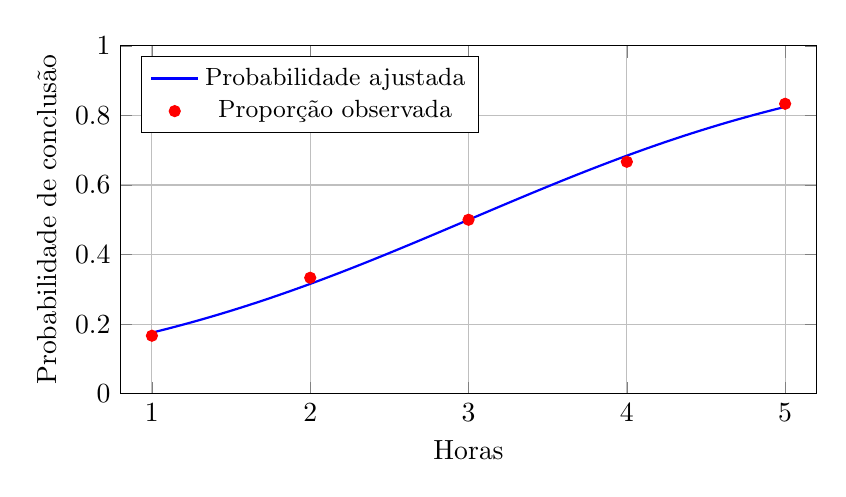
\begin{tikzpicture}
\begin{axis}[
  width=0.86\textwidth,height=6cm,
  xlabel={Horas},ylabel={Probabilidade de conclusão},
  xmin=0.8,xmax=5.2,ymin=0,ymax=1,
  xtick={1,2,3,4,5},grid=major,
  legend style={at={(0.03,0.97)},anchor=north west,font=\small}
]
  \addplot[blue,thick,domain=1:5,samples=80]
    {1/(1+exp(-(-2.32086148+0.77362049*x)))};
  \addlegendentry{Probabilidade ajustada}
  \addplot[only marks,mark=*,red] coordinates
    {(1,0.1666667) (2,0.3333333) (3,0.5) (4,0.6666667) (5,0.8333333)};
  \addlegendentry{Proporção observada}
\end{axis}
\end{tikzpicture}
\caption{Regressão logística sobre os 60 casos fictícios. Cada ponto resume 12 pessoas na mesma duração; a curva vem do ajuste individual. Elaboração própria.}
\label{fig:logistica}
\end{figure}

As probabilidades ajustadas de uma a cinco horas são aproximadamente $0{,}175$, $0{,}316$, $0{,}500$, $0{,}684$ e $0{,}825$. A presença de ambas as respostas em cada duração evita separação completa neste exemplo simples. Em outros bancos, um preditor pode separar perfeitamente os resultados e levar a coeficientes muito grandes ou problemas de convergência. Não interprete automaticamente uma OR enorme como uma estimativa precisa.

\subsection{Ajuste, classificação e limites}

O painel pode apresentar desvio, AIC e medidas como o pseudo-$R^2$ de McFadden \parencite{JamoviLogisticaCodigo}. Um pseudo-$R^2$ não é a mesma fração da soma de quadrados explicada pela regressão linear. Compare medidas entre modelos apenas quando suas definições, respostas e amostras forem compatíveis.

Transformar probabilidades em classificações exige escolher um limiar. Com limiar 0,50, uma pessoa com probabilidade 0,49 recebe uma categoria diferente de outra com 0,51, apesar da pequena diferença entre elas. Sensibilidade e especificidade condicionam a avaliação ao resultado observado; a acurácia também depende da proporção de cada resultado no banco. O limiar e as características dos casos avaliados precisam acompanhar essas medidas. A área sob a curva ROC avalia discriminação ao longo de limiares; não demonstra, sozinha, que probabilidades previstas estejam bem calibradas.

Para avaliar calibração, precisamos confrontar as probabilidades previstas e as frequências observadas em uma avaliação adequada; a documentação de calibração probabilística do scikit-learn apresenta essa distinção \parencite{SKLearnCalibracao}. Para uso preditivo real, também precisamos de dados de validação ou de um procedimento de reamostragem que considere a escolha do modelo. Os 60 casos construídos aqui servem ao ensino do ajuste, e não à validação de uma ferramenta para decidir sobre pessoas.

É possível incluir outros preditores contínuos em Covariáveis e categóricos em Fatores. Com múltiplos termos, cada OR é condicional aos demais termos do modelo e às referências escolhidas; com interações, a comparação depende também dos valores envolvidos. A relação linear exigida para um preditor contínuo é na escala do logit, e a independência das unidades precisa vir do desenho. Uma tabela binária não torna essas condições automáticas.

Um relato inicial pode ser: ``No exemplo fictício, ajustou-se uma regressão logística binária para conclusão da tarefa, evento 1 e referência 0, em função de horas. A OR por hora foi $2{,}17$, IC95\% de Wald $[1{,}38;3{,}40]$, em 60 observações independentes.'' Em uma aplicação real, acrescente as condições de obtenção dos dados, os diagnósticos, os ausentes e a avaliação compatível com a finalidade do modelo.

\subsection{Por que uma acurácia alta pode enganar?}

Vamos usar o evento Sim como positivo. Na avaliação de uma classificação, \textbf{verdadeiros positivos} (VP) são eventos previstos como Sim; \textbf{falsos negativos} (FN) são eventos previstos como Não. Entre os não eventos, \textbf{verdadeiros negativos} (VN) são previsões Não, e \textbf{falsos positivos} (FP), previsões Sim. As medidas usuais são:
\[
\text{Sensibilidade}=\frac{VP}{VP+FN},\quad
\text{Especificidade}=\frac{VN}{VN+FP},\quad
\text{Acurácia}=\frac{VP+VN}{VP+FN+VN+FP}.
\]
Imagine outro conjunto fictício com 100 pessoas, sendo cinco eventos e 95 não eventos. Uma regra que responde Não para todas acerta 95 pessoas e tem acurácia de 95\%, mas não identifica evento algum: sua sensibilidade é zero. A especificidade é 100\%. Esses números descrevem a mesma regra, com denominadores diferentes.

\begin{figure}[H]
\centering
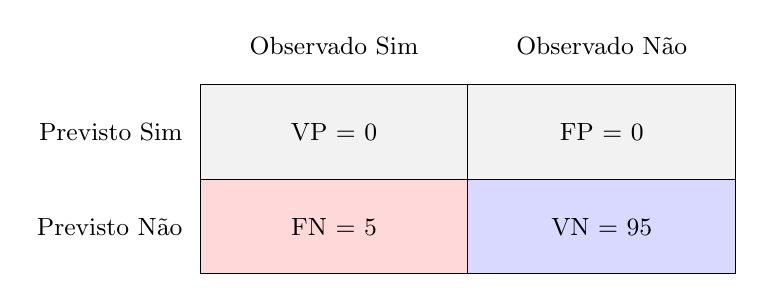
\begin{tikzpicture}[x=1cm,y=1cm,every node/.style={font=\small,align=center}]
  \node at (1.7,2.9) {Observado Sim};
  \node at (5.1,2.9) {Observado Não};
  \node[left] at (-0.1,1.8) {Previsto Sim};
  \node[left] at (-0.1,0.6) {Previsto Não};
  \fill[gray!10] (0,1.2) rectangle (6.8,2.4);
  \fill[red!15] (0,0) rectangle (3.4,1.2);
  \fill[blue!15] (3.4,0) rectangle (6.8,1.2);
  \draw (0,0) rectangle (6.8,2.4);
  \draw (3.4,0) -- (3.4,2.4);
  \draw (0,1.2) -- (6.8,1.2);
  \node at (1.7,1.8) {VP = 0};
  \node at (5.1,1.8) {FP = 0};
  \node at (1.7,0.6) {FN = 5};
  \node at (5.1,0.6) {VN = 95};
\end{tikzpicture}
\caption{Matriz de uma regra hipotética que classifica todos como Não. O acerto global de 95\% convive com falha em todos os cinco eventos. Este exemplo não é a saída do ajuste logístico do CSV. Elaboração própria.}
\label{fig:classificacao-majoritaria}
\end{figure}

Se mudarmos apenas a proporção de eventos, mantendo sensibilidade e especificidade, a acurácia muda. O valor preditivo positivo, $VP/(VP+FP)$, também depende da frequência de eventos na população avaliada; nessa regra sem qualquer previsão positiva, ele não é calculável porque o denominador é zero.

No exemplo de regressão logística, explique como o limiar foi escolhido e em quais dados as medidas foram avaliadas. Um limiar adequado depende da pergunta e das consequências das duas direções de erro. Se ele for escolhido e avaliado nos mesmos casos, a avaliação poderá ser otimista. A discussão de calibração acima acrescenta outra pergunta: se o modelo prevê probabilidades de 20\%, elas correspondem a frequências próximas de 20\% em observações comparáveis?

\section{Vamos praticar: perguntas e comentários}

\begin{enumerate}
  \item Em 52 respostas Sim de 80, qual é a proporção? Compare-a com uma referência de 50\% sem confundir proporção e valor de $p$.
  \item Uma variável com três categorias e proporções de referência iguais pede um teste de aderência ou uma tabela de independência entre duas variáveis?
  \item No exemplo pareado, quantas pessoas mudaram de Não para Sim e quantas fizeram a mudança inversa? Por que só comparar os totais marginais não descreve todos os pares?
  \item Uma OR de $2{,}17$ por hora significa que a probabilidade aumenta 117 pontos percentuais?
  \item Um resíduo positivo de A/Sim indica que a contagem observada é maior ou menor que a esperada sob independência?
  \item Uma classificação pode ter acurácia de 95\% e sensibilidade zero? Explique usando a figura~\ref{fig:classificacao-majoritaria}.
\end{enumerate}

\subsection*{Comentários das respostas}

\begin{enumerate}
  \item A proporção é $0{,}65$, ou 65\%. O teste binomial bilateral contra $0{,}50$ fornece $p\approx0{,}00968$; esse valor não é a probabilidade de a hipótese nula ser verdadeira.
  \item Um teste de aderência, pois temos uma variável e uma distribuição de referência. Para duas variáveis cruzadas, a pergunta seria outra.
  \item Dezesseis mudaram de Não para Sim e quatro de Sim para Não. Os totais marginais mostram o saldo, mas ocultam quantas pessoas mudaram em cada sentido; os pares discordantes sustentam McNemar.
  \item Não. A OR multiplica as chances. No exemplo, passar de três para quatro horas muda a probabilidade ajustada de 50\% para aproximadamente 68,4\%, segundo o modelo.
  \item Maior. O sinal acompanha $O-E$; a magnitude padronizada depende também da definição e do denominador usados.
  \item Sim. Prever Não para todas as 100 pessoas acerta os 95 não eventos, mas perde os cinco eventos. Os denominadores e a finalidade da avaliação precisam ser apresentados.
\end{enumerate}

\section{Para continuar no Balaio Científico}

Para rever as contagens e a escolha dos denominadores, leia \href{https://www.balaiocientifico.com/2026/10/dados-categoricos-no-jamovi-frequencias.html}{Dados categóricos no Jamovi: frequências, percentuais e associações}.

Para localizar a análise de tabelas na interface, veja \href{https://www.youtube.com/watch?v=z_NvuE6S14Q}{Jamovi - Tabelas de Contigência no Jamovi - Aula 17}.

\textbf{Vamos praticar:} Abra \texttt{exemplo\_frequencias.csv}, use \texttt{frequencia} em Contagens e confirme o total de 100. Relate o percentual de Sim dentro de cada grupo e o percentual do grupo A entre as respostas Sim, identificando os dois denominadores.
